\begin{CJK}{Bg5}{bsmi}

%---------------------------------------------
%	Chapter System Architecture
%---------------------------------------------

\chapter{System Architecture}

This chapter is going to explain the new design in more details. This scheme is based on DSA and it will be explained in the first section. The second section exhibits the user flow in three phases: \emph{register}, \emph{login} and \emph{verification}.

\section{System Overview}

Let us recall the authentication process about the password-based scheme. As the fig~\ref{fig:password-based-flow} shows, the user gives his username and password to the server, note that the password must to be encrypted because of the security issue. It is dangerous if the private information is transmited in plain text. Then the verification server will check whether the username, password pair is valid according to its database and return the result back to user. Figure~\ref{fig:my-scheme-flow} is the authentication process of the new scheme. Because the verification server is a passive element, clients should send a login request at first. The server will send a nonce, which is composed by the server information and some random bits, back to the client after receive a login request. The client then generates a signature for this nonce and send it to the server. At last, The server uses the corresponding public key to check whether the client is valid or not.

In comparison to the password-based scheme, this new scheme needs two extra steps. But it is not a big flaw due to the high data transfer speed by NFC technique. According to this concept, the advantage is that the data communicated between the client and the server doesn't need to be encrypted. The only \emph{secret} is private key, which is stored in client's storage. The disadvantage of this scheme is that users will need to hold a device for creating signature and help them managing their public keys. The next section will offer introduction for each components.
\begin{figure}
\centering
\subfigure[password-based scheme]{
\label{fig:password-based-flow}
\includegraphics[scale=0.6]{picture/password-based-flow.png}
}
\subfigure[my scheme]{
\label{fig:my-scheme-flow}
\includegraphics[scale=0.6]{picture/basic-idea-flow.png}
}
\caption{Authentication flow}
\end{figure}

\begin{figure}
\centering
\includegraphics[scale=0.65]{picture/final-flow.png}
\caption{Authentication flow with mobile device}
\label{fig:final-flow}
\end{figure}

\section{Components and Data flow}

\begin{figure}
\centering
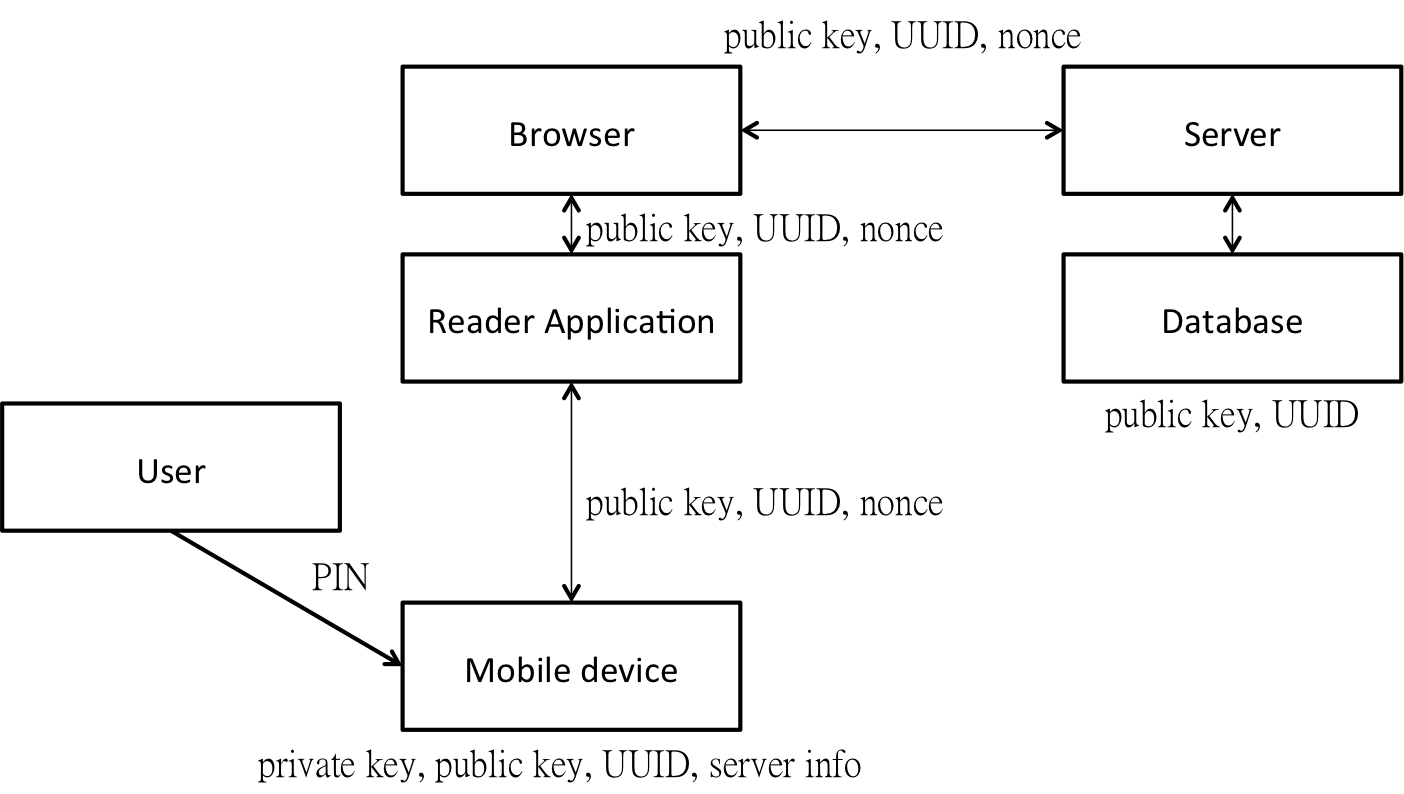
\includegraphics[scale=0.45]{picture/system-component.png}
\caption{System components}
\label{fig:system-component}
\end{figure}

As the fig~\ref{fig:system-component} shows, there are five parts of this scheme: \emph{mobile device}, \emph{NFC reader application}, \emph{browser}, \emph{srever} and the \emph{database}. The following sections will introduce the envienment where this system sets.

\subsubsection{Mobile Device and NFC Channel}

For the mobile device, this study used Nesus7 with Android OS (with Android version 4.4) in the experiments. Android OS provide a \emph{HostApduService} for developers to manage the NFC communication. Specifically, Android 4.4 supports emulating cards that are based on the NFC-Forum ISO-DEP specification (based on ISO/IEC 14443-4) and process Application Protocol Data Units (APDUs) as defined in the ISO/IEC 7816-4 specification. The protocol stack shows as fig~\ref{fig:protocol-stack}. When the user taps a device to a NFC reader, the Android system needs to know which HCE service the NFC reader actually wants to talk to. This is where the ISO/IEC 7816-4 specification comes in: it defines a way to select applications, centered around a 16-bytes Application ID (AID).

\begin{figure}
\centering
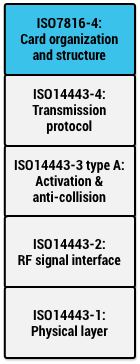
\includegraphics[scale=0.7]{picture/protocol-stack.png}
\caption{Android's HCE protocol stack\cite{nfc-hce-stack}}
\label{fig:protocol-stack}
\end{figure}

\subsubsection{Browser{
In the setup of this new scheme, it doesn't need a specify browser. Some common browsers such as Google Chrome, FireFox or IE can support this scheme.

\subsubsection{NFC Reader}
The NFC reader used in the experiments is ACR122U. The browser connect to NFC reader through Libnfc\cite{libnfc}, a open-source library for developing NFC-related application.

\subsubsection{Server and Database}

This study uses 'flask', a simple python web application framework, to build an verification server in order to proof the concept. It choose to use SQLite database, that means this scheme are compatible to password-based scheme. I use HTTPS as the transmission protocol with self-signed certificate to imitate the behavior in real world.

\section{User Flow}

This section will separate the authentication process into three stages: \emph{register phase}, \emph{login phase} and \emph{verification phase}.

\subsubsection{Register Phase}

\begin{enumerate}
\item Start the initialization process on his mobile device, that is, set PIN code and generate key pair.

Users need to set a PIN code in order to resist to thefting attack. The key pair is generated by RSA in the implementation, but it can be replaced with any other digital signature algorithm.

\item User send a registration request to the verification server.
\item Server return the server information to user and pass it to mobile device via reader application.

The reason why the server has to add server information into the nonce is to resist to the phishing attack. The mobile will show this information in its screen and users can check whether the server information (ex: url) is correct or not.

\item Mobile device saved the server information and the private key together, and return the device UUID and corresponding public key back to user.

The reason why it used the device UUID as the identifier instead of the public key is because there are various kinds of DSA. Different server can adopt different algorithm. Thus, using UUID as the identifier can unite the ID format for all the users, devices and servers.

\item User send the id and public key (and other required credentials required by server) to server.
\item Server saved UUID and public key into its database.
\end{enumerate}

\subsubsection{Login Phase}

\begin{enumerate}
\item User send a login request to server.
\item Server return a nonce ([server info || timestamp || random bits]) back to client.
\item The NFC reader start to scan cards as soon as it receive the nonce.

Notice that users have to swipe their device to the NFC reader in 30 seconds right after the reader start scanning. Otherwise, it will send a timeout message to browser.

\item User select which verification server he wants to login.
\item User execute the card emulation application on mobile device and enter the PIN code. If the PIN code correct, mobile device enable the HCE mode.
\item Reader application send nonce to mobile device
\item Mobile device retrieve the server information from nonce and check whether equal to the one user selected.
\item Mobile device signed the nonce with corresponding private key.
\item Mobile device pass its UUID and signed-nonce to reader.
\item Client pass these parameters to server.

In this step, verification server is able to ask user to provide some other credentials, but we will not discuss about that because it is not defined in the scheme.

\end{enumerate}

\subsubsection{Verification Phase}

\begin{enumerate}
\item Server retrieve the corresponding public key according to the UUID.
\item Verify the signature with the public key.
\item Return the verification result back to client.
\end{enumerate}

\section{Demonstration}



\begin{comment}
\section{Scenario}

\subsection{Future Website}
\label{sec:future-website}

\subsection{Existing Website}

For existing website, it is difficult for them to integrate this scheme with their origin users. Therefore, they can adopt the OpenID protocol to help. Build a verification server with this new scheme and use it to be the \emph{Relying Party} in OpenID protocol.

Take Bitcucket.org as an example, I modified the verification server in section~\ref{sec:future-website} to be an \emph{openid-provider}, that is, to support OpenID feature. When a user need to login to Bitbucket, he have to switch to openid-login mode, enter the server url. Then the authentication process is as same as I described above. 
\end{comment}

\end{CJK}